\documentclass[11pt,letterpaper]{article}

\usepackage[spanish,es-tabla,es-nodecimaldot]{babel}
\usepackage{amsmath}
\usepackage[utf8]{inputenc}
\usepackage[T1]{fontenc}
\usepackage{lmodern}
\usepackage{graphicx}
\usepackage{listings}
\usepackage{anysize} 
\usepackage{fancyhdr}
\usepackage{amsmath}
\usepackage{pdfpages}
\usepackage{graphics}
\usepackage{capt-of}
\usepackage{tabularx}
\usepackage{rotating}
\usepackage{tikz}
\usepackage[colorlinks=true,plainpages=true,citecolor=blue,linkcolor=blue]{hyperref}

\marginsize{2cm}{2cm}{2cm}{2cm}
\pagestyle{fancy}
\fancyhf{Sistemas celulares}
\fancyhead[L]{\footnotesize UPIITA-IPN} 
\fancyhead[R]{\footnotesize 2TV7} 
\fancyfoot[R]{\footnotesize Tarea}
\fancyfoot[C]{\thepage}
\fancyfoot[L]{\footnotesize } 

\renewcommand{\footrulewidth}{0.4pt}
\renewcommand{\spanishtablename}{Tabla}
\renewcommand{\labelitemii}{$\star$}

\graphicspath{ {C:/Users/Anselmo/Documents/GitHub/upiita-SistemasCelulares/Tarea5/imagenes} }

\begin{document}
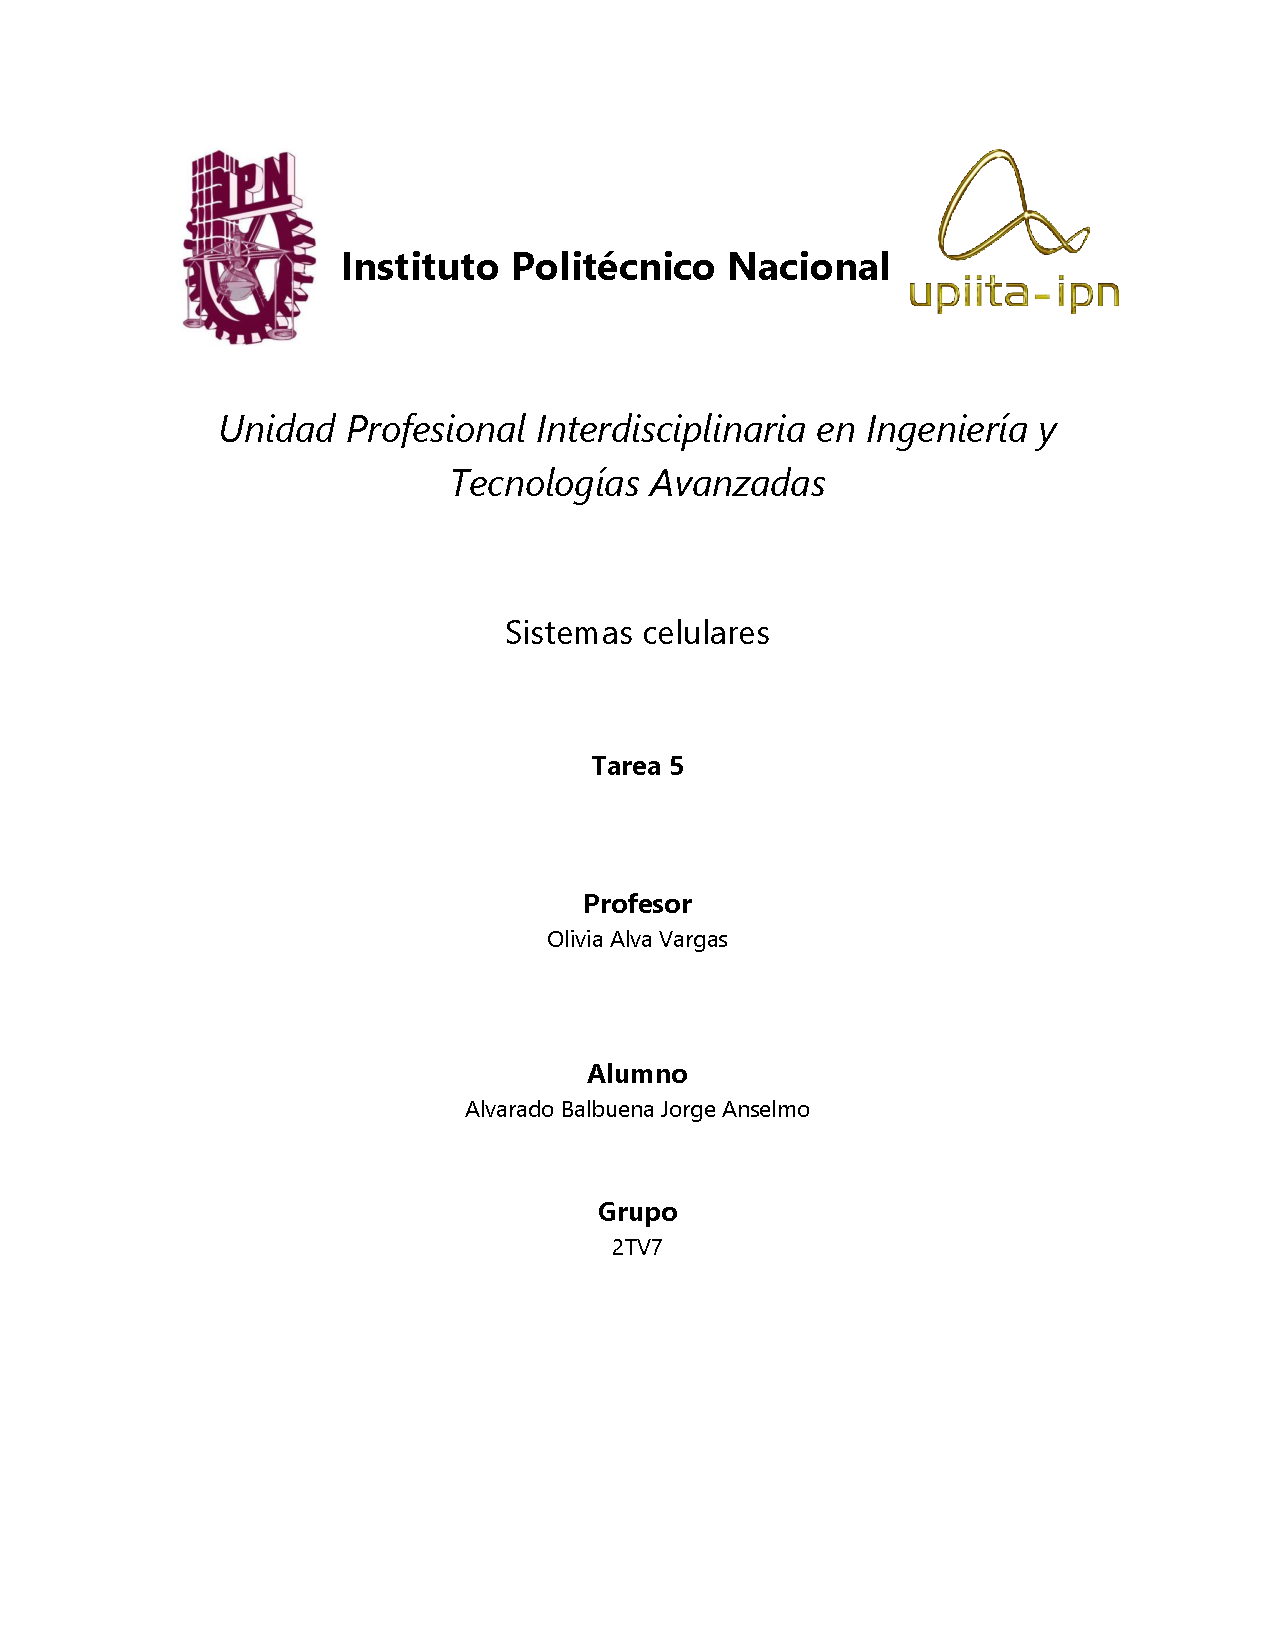
\includepdf[pages={1}]{Portada}

\newpage
\tableofcontents
\listoffigures
%\listoftables

\newpage
\section{Antecedentes}
\subsection{Códec}
Un códec es un dispositivo de hardware o un proceso basado en software que comprime y 
descomprime grandes cantidades de datos utilizados en medios de voz sobre IP, 
videoconferencia y streaming. Un códec toma datos de una forma, los codifica en otra y los 
decodifica en el punto de salida de la sesión de comunicaciones.
\\ \\
Un códec se utiliza ahora más comúnmente para describir el proceso de codificación de la 
fuente de voz y vídeo capturado por un micrófono o una cámara de vídeo en forma digital 
para su transmisión a otros participantes en llamadas, videoconferencias y transmisiones 
o emisiones. En este ejemplo, el término códec significa compresión/descompresión.
\\ \\
El trabajo principal de un códec es la transformación y encapsulación de datos para su 
transmisión a través de una red. Los códecs de voz y vídeo utilizan un algoritmo de 
software que se ejecuta en un procesador común o en hardware especializado optimizado 
para la encapsulación y decapsulación de datos.

\subsection{G.729}
G.729 es un estándar para los proveedores de centrales telefónicas privadas (PBX) con 
protocolo Internet (IP), así como para la red telefónica pública conmutada (RTPC). G.729 
digitaliza señales de voz analógicas que producen una salida a 8 kilobits por segundo (Kbps) 
con compresión 8:1 y emplea un algoritmo llamado predicción lineal excitada por código 
algebraico de estructura conjugada (CS-ACELP).
\\ \\
G.729 tiene varias extensiones o anexos. Los dos más comunes son G.729A y G.729AB. 
En G.729A, las tramas de entrada tienen una duración de 10 milisegundos (10 ms) y las 
tramas generadas contienen 80 bits. La entrada y la salida contienen muestras de modulación 
de código de pulsos de 16 bits (PCM) convertidas de o a datos comprimidos de 8 Kbps. 
El retardo algorítmico total es de 15 ms. En G.729AB, los parámetros son los mismos que 
en G.729A, con la adición de la detección de activación por voz (VAD), en la que el ancho 
de banda de la señal efectiva se reduce cuando no hay entrada de audio. Una tecnología 
conocida como generación de ruido de confort (GNC) produce una pequeña cantidad de ruido 
rosa de fondo durante las pausas en el habla para evitar la distracción del usuario que 
puede ser causada por intervalos de silencio absoluto.

\subsection{Detección de activación de voz (VAD)}
La detección de activación de voz (VAD) es una aplicación de software que permite a una 
red de datos que transporta tráfico de voz a través de Internet detectar la ausencia de 
audio y conservar el ancho de banda evitando la transmisión de paquetes silenciosos a 
través de la red. La mayoría de las conversaciones incluyen un 50\% de silencio; el VAD 
(también llamado supresión de silencio) puede habilitarse para monitorizar señales 
de actividad de voz, de modo que cuando se detecta silencio durante un tiempo determinado, 
la aplicación informa al protocolo de voz en paquetes e impide que la salida del 
codificador sea transportada a través de la red.
\\ \\
La detección de activación por voz también se puede utilizar para reenviar las 
características de ruido de ralentí (a veces llamado ruido ambiental o de confort) a 
un teléfono IP remoto o a una pasarela. El estándar universal para voz digitalizada, 
64 Kbps, es una velocidad de bits constante, ya sea que el hablante esté hablando 
activamente, esté haciendo una pausa entre pensamientos o esté totalmente en silencio. 
Sin el ruido de ralentí que da la ilusión de un flujo de transmisión constante durante 
la supresión del silencio, es probable que el oyente piense que la línea se ha cortado.

\subsection{CRTP}
El Protocolo de transporte en tiempo real (RTP) es un estándar de protocolo de Internet 
que especifica una forma en que los programas pueden gestionar la transmisión en tiempo 
real de datos multimedia a través de servicios de red unicast o multicast. Originalmente 
especificado en la Solicitud de Comentarios (RFC) 1889 del Internet Engineering Task 
Force (IETF), el RTP fue diseñado por el Grupo de Trabajo de Transporte de Audio-Video 
del IETF para soportar videoconferencias con múltiples participantes geográficamente 
dispersos. El RTP se utiliza comúnmente en aplicaciones de telefonía por Internet. RTP 
no garantiza por sí misma la entrega en tiempo real de datos multimedia (ya que esto 
depende de las características de la red); sin embargo, sí proporciona los medios para 
gestionar los datos a medida que éstos llegan a su destino de la mejor manera posible.
\\ \\
RTP combina su transporte de datos con un protocolo de control (RTCP), que permite 
supervisar la entrega de datos para grandes redes de multidifusión. La monitorización 
permite al receptor detectar si hay alguna pérdida de paquetes y compensar cualquier 
fluctuación de retardo. Ambos protocolos funcionan independientemente de la capa de 
transporte subyacente y de los protocolos de la capa de red. La información en el 
encabezado RTP le dice al receptor cómo reconstruir los datos y describe cómo se 
empaquetan los flujos de bits del codec. Como regla general, RTP se ejecuta sobre el 
Protocolo de Datagrama de Usuario (UDP), aunque puede utilizar otros protocolos de 
transporte. Tanto el protocolo de inicio de sesión (SIP) como el H.323 utilizan RTP.

\newpage
\section{Desarrollo}
El número de clúster resultantes del análisis de la tarea 3 son 2. El primer clúster 
cuenta con 7 células y el segundo con 6.

\begin{figure}[ht]
    \centering
    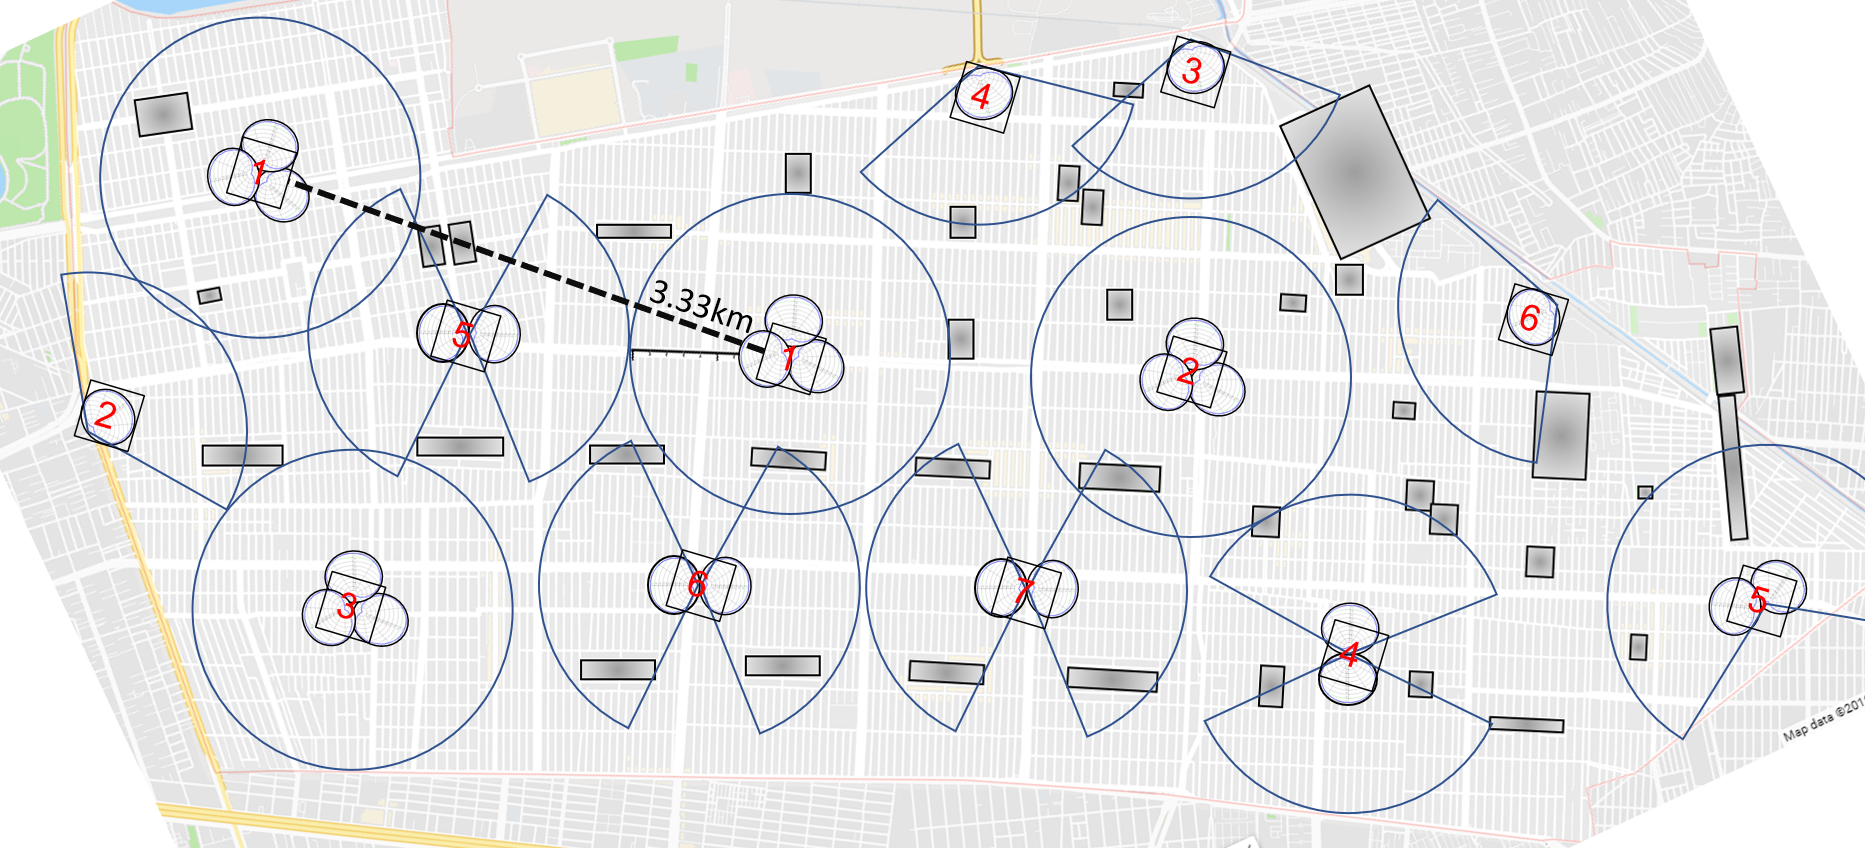
\includegraphics[width=.95\textwidth]{imagenes/t50.png}
    \caption{Área de estudio.}
\end{figure}

El sistema GSM esablece que el ancho de banda es de 60 MHz y que además se subdivide en 
canales de 200 KHz, es así que existen 300 canales que se subdividen en circuitos para 
transitar voz y/o datos considerando la Velocidad de transmisión de Voz digitalizada, 
misma que será elástica según los servicios solicitados por el usuario.
\\ \\
Algunos de estos servicios son:
\begin{itemize}
    \item Llamada en espera.
    \item Buzón de voz.
    \item Desvío de llamadas.
    \item Conferencia.
    \item Bloqueo de llamadas.
    \item Transferencia.
\end{itemize}

%El sistema GSM usa la codificación de voz G729 con muestras de 20 ms. 

\newpage
Utilizando los datos anteriores, se calcula el número de circuitos por clúster con la 
siguiente expresión.

\begin{equation}
    CH=\frac{BW_{Sis}}{BW_{CHS}}=\frac{60MHz}{200KHz}=300 \ canales
\end{equation}
\\
Con este resultado se observa que, para el área de estudio de Nezahualcóyotl, la cual tiene dos 
clústers, se cuenta con un total de 600 canales.
\\ \\
La cantidad de bits con los cuales se codifica la voz en G729, con muestras de 20ms y 
protocolo VAD es 7280 bps.

\begin{equation}
    BW_{VAD}=\eta_{TDMA}*VAD=2400*7280=17.472Mbps.
\end{equation}

\begin{equation}
    BW_{Control}=BW_{VAD}+10\%=17.472Mbps*1.10=19.2192Mbps
\end{equation}

\begin{equation}
    BW_{Tráfico}=BW_{Control}+300000=19.5192Mbps
\end{equation}

\begin{equation}
    BW_{\frac{final}{clúster}}=BW_{Tráfico}+25\% \ (CISCO)=19.5192Mbps*1.25=24.399Mbps
\end{equation}
\\ 
Así que para un clúster el ancho de banda calculado es de $24.399Mbps$, por lo que para el 
área de estudio es un total de:
\begin{equation}
    2 \ clúster * 24.399Mbps=97.356Mbps
\end{equation}
\\
Debido al cambio del ancho de banda del sistema a $60MHz$ se requiere calcular de nuevo la 
eficiencia espectral con un GoS de 99.8\%.
\\ \\
\begin{equation}
    \frac{100-GoS}{100}=\frac{100-99.8}{100}=0.002
\end{equation}
$n=301 => A=264.18 \ Erlnag$
\\ 
$n_{TDMA}=1342->A_c=1177.839 \ Erlnag$
\\ \\
$A_{TDMA}$=1177.839 Erlnag
\\ \\
Para la eficiencia espectral con los siguientes nuevos datos.
\begin{itemize}
    \item $BW_{CH}$: 200kHz = 0.2MHz.
    \item $BW_{Sis}$: 60MHz.
    \item Área: 46.74$km^2$.
\end{itemize}
Ahora sustituyendo los datos anteriores en las expresiones de la eficiencia espectral. 
\begin{equation}
    \eta=\frac{1}{BW_{CH}*N_C*Área}=\frac{1}{60*2*46.74}=178.291\mu[CH/MHz/km^2]
\end{equation}
\begin{equation}
    \eta=\frac{A \ Erlang}{BW_{Sis}*Área}=\frac{1177.839}{24*46.74}=1.049 [Erlang*MHz*km^2]
\end{equation}


\end{document}